%===================================================================================================
%  Chapter : ベクトル
%  説明    : ベクトルの考え方と計算方法を確認する.
%===================================================================================================
%   %==========================================================================
%   %  Section : ベクトルの定義
%   %==========================================================================
        \section{ベクトルの定義}
%       %----------------------------------------------------------------------
%       %  Input
%       %    File Name : PhysNote_Math_Vector_def.tex
%       %    説明      : ベクトルを定義する
%       %----------------------------------------------------------------------
        %   %==========================================================================
%   %  Section : ベクトルの定義
%   %==========================================================================
        %==================================================================
        %  SubSection
        %==================================================================
            \subsection{図形的(幾何学的)なベクトル}
                物理を考える上で,\textbf{矢印} はとても有用である.
                力の方向と大きさを直感的に表現するのに,矢印は欠かせない.
                この矢印は,数学的に扱うことができて,数学の世界では,
                矢印のことを \textbf{ベクトル} とよんでいる.

                矢印のトンガリがない方を,矢印の \textbf{始点} といい,
                トンガっている方を,矢印の \textbf{終点} という.
                これにより,方向は矢印の向きで表現できるし,その大きさは
                長さに比例するように描くと約束すれば,大きさも表現できる.
                イメージは,図\ref{fig:yajirusi_vector}に描いたようになる
                    \footnote{
                        当たり前すぎて,描くまでもなかったかな.
                    }.
                        \begin{figure}[hbt]
                            \begin{center}
                                \includegraphicsdefault{yajirusi_vector.pdf}
                                \caption{ベクトル:図形,矢印}
                                \label{fig:yajirusi_vector}
                            \end{center}
                        \end{figure}

                これを文字で表すと,始点を $\mathrm{O}$ とし,また,終点を $\mathrm{P}$ とする
                線分 $\overline{\mathrm{OP}}$ に向きをつけたと考えて,
                    \begin{equation*}
                        \overrightarrow{\mathrm{OP}}
                    \end{equation*}
                と書ける.

            \begin{memo}{ベクトルの位置は不問である}
                同じ大きさで,同じ向きをもつベクトルがいくつか存在する
                場合を考える.これらのベクトルの位置が異なる場合,
                異なるベクトルと考えるべきなのだろうか.
                        \begin{figure}[hbt]
                            \begin{center}
                                \includegraphicsdefault{OnajiVector.pdf}
                                \caption{ベクトル:図形,矢印}
                                \label{fig:OnajiVector}
                            \end{center}
                        \end{figure}

                結論から書くと,これらのベクトルは,同一とみなされる.
                つまり,ベクトルの存在する場所は,そのベクトルの性質
                には何ら関係がないということだ.そもそも,ベクトルと
                は大きさと向きのみをもつ概念であるから,当然,ベクトルが
                同一であるということは,大きさと向きが同じであるということ
                である.ベクトルが存在する場所は,定義には含まれておらず,
                不問とされるのである.

                ベクトルという概念は,力学を数式化するために整備されたものである.
                ベクトルを用いることで,物体にかかる力を数式で表現できるように
                なるのだ.例えば,自分が誰かから引っ張られる場合を想像してみよう.
                同じ大きさの力で,同じ向きに引っ張られるのであれば,引っ張られる
                場所は関係ない.引っ張られる場所が,公園だろうが,公民館だろうが,
                あるいはトイレだろうが,引っ張られるときの感覚は同一のはずである.
                つまり,力そのものは,その発生場所には関係がないのである.ベクトル
                という概念は力学の記述に適するようにつくられたので,力と同様に,
                その存在する場所には依存しないのである.というか,依存しないと定義
                付けるのである
                    \footnote{
                        ベクトルの定義では,場所に依存しないという直接的な記述はないが,
                        定理として成り立つ性質として,このことが保証される.場所に
                        依存しないように定義付けを行っているんだから,当たり前だ.
                    }.
                いつどんな場所でも,
                同じ物体に同じ力をかければ,その位置の変化の仕方もまた同じなのである.
                いや,結果が同じになるように,ベクトルという概念を定義してしまうのだ.
            \end{memo}

        %==================================================================
        %  SubSection
        %==================================================================
            \subsection{代数的なベクトル}
            \begin{mycomment}
                ベクトルを数式で扱えるように,是非とも,
                文字を使ってベクトルを表現したい.
                ベクトルは代数的に表現可能なのだが
                    \footnote{
                        「代数的に表現可能」とは,文字の列として表現
                        することが可能であるということである.
                    },
                2つの書き方がある.書き方の違いにより,次のように
                言葉を割当て,区別する.すなわち,
                    \begin{itemize}
                        \item 横ベクトル
                        \item 縦ベクトル
                    \end{itemize}
                なぜこう言われるかは,後の記述で分かることなので,
                今は気にせず,話を進めよう.
                横ベクトル$\cdot$縦ベクトル共に,どちらも同じように頻繁に使われる.
                どっちも大切である.どちらか一方を採用したら,他方を捨て去るということ
                はない.
            \end{mycomment}

            %==============================================================
            %  SubsubSection
            %==============================================================
                \subsubsection{横ベクトル}
                ベクトルを代数的に表現する方法は2通りあると,先に記述した.
                ここではそのうちの,\textbf{横ベクトル} について,説明する.

                ベクトルをどのように代数的に表現するのか.実は,
                その考え方は簡単で,そのベクトルの始点に原点 $O$ を合わせた
                座標を張ればよい.図\ref{fig:yajirusi_vector_daisu}では
                直交直線座標を描いた.これより,終点の座標を記述する
                ことで,ベクトルを表現できるのである.
                        \begin{figure}[hbt]
                            \begin{center}
                                \includegraphicsdefault{yajirusi_vector_daisu.pdf}
                                \caption{ベクトル:図形,矢印}
                                \label{fig:yajirusi_vector_daisu}
                            \end{center}
                        \end{figure}

                代数的なベクトルは,以下のように記述される.
                    \begin{align}
                        \br = \left[\,x\,,y\,\right].
                    \end{align}
                上の表現では,2次元の平面に存在するベクトルが記述されている.より高次元の
                ベクトル $\bx$ を考える場合,その次元数を $n$ として,
                    \begin{align}
                        \bx = \left[\,x_{1}\,,\,\,x_{2}\,,\,\,\cdots\,,\,\,x_{n}\,\right].
                    \end{align}
                ここで,座標を表すこ記号を,$x$ に統一して添字により区別すよう,
                表現方法を変えた.

                このように,成分を横書きしたベクトル表記を,\textbf{横ベクトル} という.

                ベクトルを表現するのに,太字を用いているのは,単なる実数と
                区別するためである.

            %==============================================================
            %  SubsubSection
            %==============================================================
                \subsubsection{縦ベクトル}
                    横ベクトルが成分を横書きしたベクトル表現だとしたら,
                    \textbf{縦ベクトル} とは成分を縦書きしたベクトル表現である.
                    なんとも安易な考え方だ.縦ベクトルは以下のように記述される.
                    \begin{align}
                        \bx
                        =
                        \left[
                            \begin{array}{c}
                                x_{1} \\
                                x_{2} \\
                                \vdots \\
                                x_{n} \\
                            \end{array}
                        \right].
                    \end{align}

        %==================================================================
        %  SubSection
        %==================================================================
            \subsection{ベクトルの大きさ}
                ベクトルの大きさは,三平方の定理により定義できる
                    \footnote{
                        三平方の定理について一言コメントしておこう.
                        これは数学的には三角関数の余弦定理の特殊な場合である.
                        しかし,ここでは,三平方の定理を距離を定めるひとつの要請
                        として扱うことにする.
                    }.

                まず,2次元ベクトル $\br=\left[\,x\,,y\, \right]$ の場合,このベクトルの
                大きさは三平方の定理によって定められ,
                    \begin{align}
                        |\br| = \sqrt{x^{2} + y^{2}}
                    \end{align}
                である.
                        \begin{figure}[hbt]
                            \begin{center}
                                \includegraphicsdefault{SanHeihouNoTeiri_2D_01.pdf}
                                \caption{三平方の定理(2次元)}
                                \label{fig:SanHeihouNoTeiri_2D_01}
                            \end{center}
                        \end{figure}

                2次元のベクトルの大きさを,3次元ベクトルに拡張しよう.
                図\ref{fig:SanHeihouNoTeiri_3D_01}の色を塗った部分の
                直角三角形に着目する.このとき,2次元の三平方の定理から,
                    \begin{equation*}
                        |\br| = \sqrt{\left(\sqrt{x^{2} + y^{2}}\right)^{2} + z^{2}}
                    \end{equation*}
                が成立している.つまり,
                    \begin{align}
                        |\br| = \sqrt{{x}^{2} + {y}^{2} + {z}^{2}}
                    \end{align}
                という関係があるということだ.もはや変数は4つであり,
                "三平方"という語彙と食い違ってしまったが,とりあえず,
                ここでは,3次元の三平方の定理と表現しておこう.
                        \begin{figure}[hbt]
                            \begin{center}
                                \includegraphicslarge{SanHeihouNoTeiri_3D_01.pdf}
                                \caption{三平方の定理(3次元)}
                                \label{fig:SanHeihouNoTeiri_3D_01}
                            \end{center}
                        \end{figure}

        %==================================================================
        %  SubSection
        %==================================================================
            \subsection{ベクトルの次元}
            私たちは,3次元の世界に住んでいるから,当然,縦$\cdot$横$\cdot$高さ
            の3方向しか把握できない.4つ以上の次元で成り立つ世界を見ることは
            不可能である.しかし,数学的には,4つ以上の方向を考えても,理論的
            に矛盾することはない.つまり,数学的には,より多くの方向をもつベクトルを
            扱えるのである
                \footnote{
                    ただし,4つ以上の方向を肌で感じたり,見たりできない以上,
                    図示することは不可能であるから,4次元以上の世界は完全に
                    文字(数式)だけの記述のみになってしまう.
                }.
            そこで,4つ以上の方向をもつベクトルについて,考える.

            まず,今まで日常生活的に使用してきた,\textbf{次元} という語彙を,
            数学用語として改めてその意味を明確にしておきたい.次元とは,ベクトルの
            成分の個数と定める.ただし,物理学では単位のことを次元と表現するが
                \footnote{
                    物理学では「次元解析」という言葉が使われる.これは,物理学的な単位
                    同士の関係を調べることであり,特に,数式の右辺と左辺の単位に矛盾が
                    ないかを確認することで利用される.しかし,ここで考えている次元とは,
                    意味が異なる(完全に異なるわけではないが)ものとして,考えてもらいたい.
                    少なくとも,いま考える次元とは,空間の方向の数であり,ベクトルの
                    成分の個数のことである.
                },
            それとは別物である.

            あるベクトル $\br$ があり,その成分が $n$ 個であるとしよう.つまり,
                \begin{equation*}
                    \br = \left[r_{1},\,r_{2},\,r_{3},\,\cdots,\,r_{n}\right]
                \end{equation*}
            と成分表示されるとする.この時,$\br$ のことを \textbf{$n$ 次元ベクトル} と
            いう.

                \begin{memo}{$n$ 次元の三平方の定理}
                    2次元と3次元の両方の三平方の定理から推察して,
                    より高次元である $n$ 次元に定理を拡張できる.
                    もちろん,$n$ は任意の自然数である.
                    この拡張に伴って,この定理に改めて名前をつける
                    ことにしよう
                        \footnote{
                            これから定義しようとするのは,$n$ 次元での定理
                            であり,それには $n+1$ 個の数が絡んでくるから,
                            「三平方の定理」では定理の内容と一致しなくなってしまう
                            のだ.
                        }.
                    \textbf{距離の公理} と名付ける.

                    $n$ 次元への拡張は以下のようにして行われる.
                    \begin{align}
                        r := |\br|
                           = {q_{1}}^{2} + {q_{2}}^{2} + \cdots + {q_{n}}^{2}
                           = \sqrt{\sum_{i=1}^{n} {q_{i}}^{2}}.
                    \end{align}
                    ここに,$q_{i}$ はそれぞれ座標を表す.
                \end{memo}

        %==================================================================
        %  SubSection
        %==================================================================
            \subsection{ベクトル空間の定義}
                ベクトルをより一般的に定義しておきたい.そこで,はじめに,
                ベクトルの集合を定義する.ベクトルの持つ性質を列挙して,
                それを満たすものを,\textbf{ベクトル空間} とよぶ.そして,
                ベクトルをベクトル空間の要素として定義することで,ベクトル
                を,数学的に曖昧さのない概念として,扱うことが可能になる.
                    \\
                    \begin{itembox}[l]{\textbf{ベクトル空間}}
                        \begin{dfn}
                            ある集合 $\bU$ が次の条件全てを満たすとき,$\bU$ を \textbf{ベクトル空間} という.

                                集合 $\bU$ の任意の要素 $\ba$,$\bb$,$\bc$ に対して,
                                \begin{description}
                                    \item[\;\;\;1]\;\;\; $(\ba + \bb) + \bc = \ba + (\bb + \bc) $
                                    \item[\;\;\;2]\;\;\; $\ba + \bb = \bb + \ba$
                                    \item[\;\;\;3]\;\;\; $\bo + \ba = \bo$ を満たす $\bo$ がただ一つ存在する.
                                    \item[\;\;\;4]\;\;\; $\ba + \ba' = \bo$ を満たす $\ba'$ がただ一つ存在する.
                                \end{description}
                                が成立する.

                                さらに,任意の実数 $m$,$n$ に対して,
                                \begin{description}
                                    \item[\;\;\;5]\;\;\; $(m + n) \ba = m\ba + n\ba$
                                    \item[\;\;\;6]\;\;\; $m( \ba + \bb )$
                                    \item[\;\;\;7]\;\;\; $(mn)\ba = m(n\ba)$
                                    \item[\;\;\;8]\;\;\; $1\ba = \ba$
                                \end{description}
                                が成立する.

                            特に,$\bo = (\,0,\,0,\, \cdots,\,0\,)$ であり,\textbf{ゼロベクトル} という.
                        \end{dfn}
                    \end{itembox}
                    \\

        %==================================================================
        %  SubSection
        %==================================================================
            \subsection{ベクトルの定義}
                ベクトルを定義しよう.
                \\
                \begin{itembox}[l]{\textbf{ベクトル}}
                    \begin{dfn}
                        ベクトル空間 $\bU$ の要素のことを \textbf{ベクトル} という.
                    \end{dfn}
                \end{itembox}
                \\


%   %==========================================================================
%   %  Section : ベクトルの性質
%   %==========================================================================
        \section{ベクトルの性質}
%       %----------------------------------------------------------------------
%       %  Input
%       %    File Name : PhysNote_Math_Vector_AddSubMul.tex
%       %    説明      : ベクトルの加法,スカラー倍などを説明する
%       %----------------------------------------------------------------------
                %======================================================================
        %  SubSection
        %======================================================================
        \subsection{ベクトルの転置}
            横ベクトルと縦ベクトルの関係を,ここに書いておこう.
            議論の最初に,横ベクトルで表現したベクトルを,縦ベクトル
            として表現したい場合が起こる
                \footnote{
                    特に,ベクトルの内積を行列的に記述したい場合に,
                    このような要求をしたくなる.
                }

            そんな時,活躍するのが,ベクトルの \textbf{転置} という
            考え方である.

            $n$ 次元ベクトル $\bx$ を最初に導入するとき,
            横ベクトルとして定義したとする.そして,議論の途中,
            $\bx$ を縦ベクトルとして記述したくなったとしよう.
            すなわち,以下のような書き換えたいのである.
            \begin{align*}
                \left[\,x_{1}\,,\,\,x_{2}\,,\,\,\cdots\,,\,\,x_{n}\,\right]
                \quad \rightarrow \quad
                \left[
                    \begin{array}{c}
                        x_{1} \\
                        x_{2} \\
                        \vdots \\
                        x_{n} \\
                    \end{array}
                \right]
            \end{align*}
            要するに,横ベクトルの成分表示で,その成分を左から順に書いていたベクトルを,
            縦に上から順に成分を記述する方式に変更したいのだ.
            この操作を,ベクトルの \textbf{転置} という.

            この場合,以下のように記述する.
            \begin{align}
                {}^{t}\left[\,x_{1}\,,\,\,x_{2}\,,\,\,\cdots\,,\,\,x_{n}\,\right]
                =
                \left[
                    \begin{array}{c}
                        x_{1} \\
                        x_{2} \\
                        \vdots \\
                        x_{n} \\
                    \end{array}
                \right].
            \end{align}

            左辺の左上の添字 ${}^{t}$ で,ベクトルの転置を表現する.

            最初に定義されたベクトルが縦ベクトルであっても,
            ベクトルの転置を行うことで,横ベクトルにできる.
            つまり,次のようにも記述して良い.
            \begin{align}
                    \begin{array}{c}
                        {}^{t}
                        \\
                        \\
                        \\
                        \\
                    \end{array}
                \left[
                    \begin{array}{c}
                        x_{1} \\
                        x_{2} \\
                        \vdots \\
                        x_{n} \\
                    \end{array}
                \right]
                =
                \left[\,x_{1}\,,\,\,x_{2}\,,\,\,\cdots\,,\,\,x_{n}\,\right]
            \end{align}

            以上から,ベクトルの転置について,次が成立している.
            \begin{align}
               {}^{t} ({}^{t}\bx) = \bx.
            \end{align}

            ベクトル $\bx$ に2回転置をすれば,元のベクトルに戻るのである.
            以下のような感じで,巡回が起こる.
            \begin{align*}
                \mbox{縦ベクトル}
                    \xrightarrow[\mbox{\small{転置}}]{} \mbox{横ベクトル}
                    \xrightarrow[\mbox{\small{転置}}]{} \mbox{縦ベクトル} \\
                \mbox{横ベクトル}
                    \xrightarrow[\mbox{\small{転置}}]{} \mbox{縦ベクトル}
                    \xrightarrow[\mbox{\small{転置}}]{} \mbox{横ベクトル}
            \end{align*}

            もちろん,横ベクトルで表現しようとも,縦ベクトルで表現
            しようとも,同一のベクトルであれば,それが示すベクトルは同一
            である.同じベクトルを表現する方法が2種類あるということであり,
            ベクトルが2つになるわけではない.$\bx$ も ${}^{t}\bx$ も同じ
            ベクトルを表現するものであり,違うのは表現の方法なのだ.

        %==================================================================
        %  SubSection
        %==================================================================
            \subsection{ベクトルの四則演算}
            \begin{mycomment}
                ここでは,ベクトルに対して四則演算を定義する.
            \end{mycomment}

            %==============================================================
            %  SubSection
            %==============================================================
            \subsubsection{ベクトルの加法}
            3次元の2つのベクトルを,任意にもってきて,それらを
            \begin{equation*}
                \bx =
                \left[
                    \begin{array}{c}
                        x_{1} \\
                        x_{2} \\
                        x_{3} \\
                   \end{array}
                \right]\quad , \qquad
                \by =
                \left[
                    \begin{array}{c}
                        y_{1} \\
                        y_{2} \\
                        y_{3} \\
                   \end{array}
                \right]
            \end{equation*}
            と書くことにしよう.
            これら2つのベクトル $\bx$,$\by$ の和 $\bx + \by$ は,成分表示で
            以下のように示される.
                    \begin{align}
                        \bx + \by
                        =
                        \left[
                            \begin{array}{c}
                                x_{1} \\
                                x_{2} \\
                                x_{3} \\
                            \end{array}
                        \right]
                        +
                        \left[
                            \begin{array}{c}
                                y_{1} \\
                                y_{2} \\
                                y_{3} \\
                            \end{array}
                        \right]
                        =
                        \left[
                            \begin{array}{c}
                                x_{1} + y_{1} \\
                                x_{2} + y_{2} \\
                                x_{3} + y_{3} \\
                            \end{array}
                        \right].
                    \end{align}

                    つまり,成分同士を足し合わせるということである.

                    $n$ 次元ベクトルに対して,拡張しておこう.
                    任意の 2つの $n$ 次元ベクトル
                    \begin{equation*}
                        \bx =
                        \left[
                            \begin{array}{c}
                                x_{1} \\
                                x_{2} \\
                                \vdots \\
                                x_{n} \\
                           \end{array}
                        \right]\quad , \qquad
                        \by =
                        \left[
                            \begin{array}{c}
                                y_{1} \\
                                y_{2} \\
                                \vdots \\
                                y_{n} \\
                           \end{array}
                        \right]
                    \end{equation*}
                    に対して,これらの和は,成分で書くと次のようになる.
                    \begin{align}
                        \bx + \by
                        =
                        \left[
                            \begin{array}{c}
                                x_{1} \\
                                x_{2} \\
                                \vdots \\
                                x_{n} \\
                            \end{array}
                        \right]
                        +
                        \left[
                            \begin{array}{c}
                                y_{1} \\
                                y_{2} \\
                                \vdots \\
                                y_{n} \\
                            \end{array}
                        \right]
                        =
                        \left[
                            \begin{array}{c}
                                x_{1} + y_{1} \\
                                x_{2} + y_{2} \\
                                \vdots \\
                                x_{n} + y_{n} \\
                            \end{array}
                        \right].
                    \end{align}

                    また,次元の違うベクトル同士の和は定義されない.
                    つまり,次元が違うと,加法を行うことはできない.

            %==============================================================
            %  SubSection
            %==============================================================
            \subsubsection{実数とベクトルの積}
                ここでは,ひとつの任意の実数と,ひとつの任意のベクトルの
                積を定義する.ベクトル同士の掛け算も定義されるが
                    \footnote{
                        ベクトルの内積$\cdot$外積を参照.
                    },
                ここでは,実数とベクトルの掛け算のみについて考える.

                任意の実数 $a$ と任意の $n$ 次元ベクトル $\bx$ をもってきて,
                積を作る.その積を,
                    \begin{equation*}
                        a\bx
                        =
                        a\left[
                        \begin{array}{c}
                            x_{1}  \\
                            x_{2}  \\
                            \vdots \\
                            x_{n}  \\
                        \end{array}
                    \right]
                    \end{equation*}
                と書くことにする.成分で書くと,次のようになる
                    \footnote{
                        というか,こうなるように,実数とベクトルの積を
                        定義する.
                    }.
                \begin{align}
                    a\bx
                    =
                    a\left[
                        \begin{array}{c}
                            x_{1}  \\
                            x_{2}  \\
                            \vdots \\
                            x_{n}  \\
                        \end{array}
                    \right]
                    =
                    \left[
                        \begin{array}{c}
                            ax_{1}  \\
                            ax_{2}  \\
                            \vdots \\
                            ax_{n}  \\
                        \end{array}
                    \right].
                \end{align}

                これは $n$ 次元ベクトルに対して成り立つものである.
                つまり,実数とベクトルの積は,ベクトルの各成分を
                実数 $a$ 倍するということである.

            %==============================================================
            %  SubSection
            %==============================================================
            \subsubsection{ベクトルの減法}
                実数の世界では,事実上,減法が存在するが,しかしこれは公理的
                視点からは加法の一部である.つまり,2つの実数 $x$,$y$ があった
                時,減法 $x-y$ は 加法 $x+(-1 \cdot y)$ で定義されるのである.
                負の記号 $-1$ は公理により,その存在が示されているからである.
                減法を新たに定義するよりも,$-1$ の存在を主張するほうが,理論が
                単純になるり,思考経済
                    \footnote{
                        \textbf{思考経済}\quad
                        同じことを説明するのに,2つ以上の手段があるとしよう.
                        思考経済とは,この2つの説明のうちどちらを採用するかという
                        基準である.「簡潔に説明できる方を採用せよ」というものだ.
                        もちろん,最も簡潔に説明するほうがいいに決まっている(直感だけど)
                        うだうだ説明するりも,スパッと説明したほうが
                        かっこいいし,覚えることも少なくすむし,何しろ短時間で
                        説明できるのだから.しかし,世の中にはどちらも同じだけ
                        簡潔に説明できることが多くある.その場合には,時と場合に
                        よって使い分ける必要が出てくることだろう.
                    }
                に合致する.

                ベクトルに関する減法も,実数と同様に,加法の一部として,説明される
                べきものである.負の向きをもつベクトルとは,当然,正の向きに対して
                逆向きのベクトルである.負の向きのベクトルは,ベクトルに $-1$ を掛
                けることで,得られる.つまり,任意の $n$ 次元ベクトル $\by$ に対して,
                これと同じ大きさで,逆向きのベクトルは,
                \begin{equation*}
                    -1 \cdot \by = -\by
                \end{equation*}
                と書かれる.実数の場合と同じように,$-1$ 倍のときは,$1$を省略して
                書くことにする.

                これを用いて,ベクトルの減法を定めよう.
                任意の 2つの $n$ 次元ベクトル $\bx$,$\by$ に対して,差
                $\bx - \by$ とは次のように,成分表示される.
                \begin{align}
                    \bx - \by &= \bx + (- \by) \notag \\
                    &=
                    \left[
                        \begin{array}{c}
                            x_{1}  \\
                            x_{2}  \\
                            \vdots \\
                            x_{n}  \\
                        \end{array}
                    \right]
                    +
                    (-1)\left[
                        \begin{array}{c}
                            y_{1}  \\
                            y_{2}  \\
                            \vdots \\
                            y_{n}  \\
                        \end{array}
                    \right] \notag \\
                    &=
                    \left[
                        \begin{array}{c}
                            x_{1}  \\
                            x_{2}  \\
                            \vdots \\
                            x_{n}  \\
                        \end{array}
                    \right]
                    +
                    \left[
                        \begin{array}{c}
                            -y_{1}  \\
                            -y_{2}  \\
                            \vdots \\
                            -y_{n}  \\
                        \end{array}
                    \right] \notag \\
                    &=
                    \left[
                        \begin{array}{c}
                            x_{1}  +(-y_{1}) \\
                            x_{2}  +(-y_{2}) \\
                            \vdots \\
                            x_{n}  +(-y_{n}) \\
                        \end{array}
                    \right] \notag \\
                    \therefore \quad
                    \bx - \by
                    &=
                    \left[
                        \begin{array}{c}
                            x_{1}  -y_{1} \\
                            x_{2}  -y_{2} \\
                            \vdots \\
                            x_{n}  -y_{n} \\
                        \end{array}
                    \right]
                \end{align}



%       %----------------------------------------------------------------------
%       %  Input
%       %    File Name : PhysNote_Math_Vector_NaiSekiGaiSeki.tex
%       %    説明      : ベクトルのもつ性質(内積など)を考える
%       %----------------------------------------------------------------------
        %   %==========================================================================
%   %  Section : ベクトルの性質
%   %==========================================================================
        %==================================================================
        %  SubSection
        %==================================================================
            \subsection{ベクトルの内積(図形的)}\label{subsec:VecNaisekiFig}
                ベクトルの内積について,簡単に説明をしておこう.

                2つの任意のベクトルを用意し,$\ba$,$\bb$ とする.ベクトルの \textbf{内積} は
                この2つのベクトルより定義される.
                内積の表し方は,$(\ba\,,\;\bb)$ または $\ba\cdot\bb$ などの複数の表現がある.
                このノートでは,$\ba\cdot\bb$ を内積の記号として使うことにする.
                ベクトルの内積を,次のように,平面図形的に定義する.
                    \\
                    \begin{itembox}[l]{\textbf{ベクトルの内積(図形的)}}
                        \begin{dfn}
                            任意の2つのベクトル $\ba$ と $\bb$ の間に,演算 $\cdot$ を
                            以下のように定義する.
                            \begin{align}
                                 \ba\cdot\bb := | \ba |  | \bb | \cos\theta
                            \end{align}
                            この演算を,ベクトル $\ba$ と $\bb$ の \textbf{内積} という.
                        \end{dfn}
                    \end{itembox}
                    \\

                この式のイメージは,「$\ba$ の $\bb$ 方向の成分の大きさ」と,$\bb$ の積の大きさである.
                    \begin{equation*}
                        \ba\cdot\bb = ( | \ba | \cos\theta ) | \bb |
                    \end{equation*}
                と書いたらイメージしやすい.$| \ba | \cos\theta$ の $|\bb|$ 倍ということである.

                    \begin{figure}[hbt]
                        \begin{center}
                            \includegraphicsdefault{bekutoru_no_naiseki.pdf}
                            \caption{内積}
                            \label{fig:bekutoru_no_naiseki}
                        \end{center}
                    \end{figure}

                例えば,$\theta = 60{}^{\circ}$,$| \ba | = 3$,$| \bb | = 5$ のとき,
                    \begin{align*}
                        \ba\cdot\bb     &= | \ba |  | \bb | \cos\theta = 3 \times 5 \times \cos(60{}^{\circ}) \\
                                            &= 3 \times 5 \times \frac{1}{2} \\
                                            &= \frac{15}{2}
                    \end{align*}
                となる.
        %==================================================================
        %  SubSection
        %==================================================================
            \subsection{ベクトルの内積(代数的)}\label{subsec:VecNaisekiArg}
                実は,ベクトルの内積には,もう一つ別の定義がある.もちろん,上に説明した平面図形的定義と
                全く矛盾しない.別の定義とは,ベクトルの成分に着目した,代数的定義である
                    \footnote{
                        「平面図形的定義」と「代数的定義」は私の造語.
                    }.

                ベクトルの内積の代数的定義は,次式で定義される.
                    \\
                    \begin{itembox}[l]{\textbf{ベクトルの内積(代数的)}}
                        \begin{dfn}
                            任意の2つのベクトル $\ba$ と $\bb$ があるとする.
                            ベクトルの成分を
                                $\ba=\left[\,a_{1},\,a_{2},\,\cdots,\,a_{n}\,\right]$,
                                $\bb=\left[\,b_{1},\,b_{2},\,\cdots,\,b_{n}\,\right]$ で
                            表すとき,この2つのベクトルの間の演算 $\cdot$ を
                            次で定義する
                                \begin{align}
                                    \ba\cdot\bb = \sum_{i=1}^{n} a_{i}b_{i}.
                                \end{align}
                        \end{dfn}
                    \end{itembox}
                    \begin{description}
                        \item[例] 仮に,2つのベクトルの成分は2つとしよう.
                        つまり,$\ba=\left[a_{1},\,a_{2}\right]$,
                                $\bb=\left[b_{1},\,b_{2}\right]$ と仮定する.
                        このときベクトルの内積は
                            \begin{align}
                                \ba\cdot\bb = a_{1}b_{1}+a_{2}b_{2}
                            \end{align}
                        である.
                    \end{description}



        %==================================================================
        %  SubSection
        %==================================================================
            \subsection{図形的内積と代数的内積の関係}
                図形的定義による内積と代数的定義による内積が全く同じことであることは,次のように説
                明できる
                    \footnote{
                        互いに矛盾する定義だったら,内積の定義としてどちらを採用するかを検討しない
                        といけない.もしくは,両方とも採用しないことになるかもしれない.だけど,全
                        く同じことを言っているのだから,都合のよい方を,定義式として採用してよいの
                        である.

                        今回は,まずイメージしやすいように図形的な定義を先に紹介した.
                        だけど,物理学の理論を考えるには,数式で表現する必要がある.
                        $\cos$ 関数を用いた図形的定義でも事足りると思うが,
                        代数的な内積の式も有用なので,紹介をしておいた.
                    }.

                2つの任意のベクトル $\ba$,$\bb$ の内積を考える.
                この2つのベクトルを直交座標の $x$ 座標,$y$ それぞれ座標の成分に分解し,
                    \begin{align*}
                        \begin{cases}
                        \displaystyle \ba = \ba_{x}  +  \ba_{y} \\
                        \displaystyle \ba = \bb_{x}  +  \bb_{y}
                        \end{cases}
                    \end{align*}
                とする.
                    \begin{figure}[hbt]
                        \begin{center}
                            \includegraphicslarge{naiseki_zahyou_zukei.pdf}
                            \caption{内積(代数的定義と図形的定義の関係)}
                            \label{fig:naiseki_zahyou_zukei}
                        \end{center}
                    \end{figure}
                ここで, $\ba$,$\bb$ の内積を図形的に計算してみよう.
                    \begin{align*}
                        \ba\cdot\bb &= ( \ba_{x}  +  \ba_{y} ) \cdot  ( \bb_{x}  +  \bb_{y} ) \\
                                        &= \ba_{x}\cdot\bb_{x} + \ba_{x}\cdot\bb_{y} +\ba_{y}\cdot\bb_{x} + \ba_{y}\cdot\bb_{y}
                    \end{align*}
                右辺の各項を,それぞれ計算しよう.($\cos {0\,}^{\circ}=1$,$\cos {90\,}^{\circ}=0$)
                    \begin{align*}
                        \begin{cases}
                        \displaystyle \ba_{x}\cdot\bb_{x} = |\ba_{x}| |\bb_{x}| \cos {0\,}^{\circ} = a_{x}b_{x}. \\
                        \displaystyle \ba_{x}\cdot\bb_{y} = |\ba_{x}| |\bb_{y}| \cos {90\,}^{\circ} = 0.\\
                        \displaystyle \ba_{y}\cdot\bb_{x} = |\ba_{y}| |\bb_{x}| \cos {90\,}^{\circ} = 0.\\
                        \displaystyle \ba_{y}\cdot\bb_{y} = |\ba_{y}| |\bb_{y}| \cos {0\,}^{\circ} = a_{y}b_{y}.\\
                        \end{cases}
                    \end{align*}
                つまり,
                    \begin{align}
                         \ba\cdot\bb = a_{x}b_{x} + a_{y}b_{y}
                    \end{align}
                である.これで,代数的定義は,図形的定義と同じこだと,分かるだろう.
                    \\
                    \begin{itembox}[l]{\textbf{ベクトルの内積}}
                        直交座標上における,
                        2つの二次元ベクトル $\ba = \left[a_{x} ,\,a_{y}\right]$,
                        $\bb = \left[b_{x} ,\,b_{y}\right]$ に対して,
                        ベクトルの \textbf{内積} $\ba\cdot\bb$を
                        次式で定義する.
                            \begin{align}
                                \ba \cdot \bb := a_{x}b_{x} + a_{y}b_{y}.
                            \end{align}

                        $n$ 次元ベクトル同士の内積の場合,
                            \begin{align}
                                \ba \cdot \bb := \sum_{i=1}^{n}a_{i}b_{i}.
                            \end{align}
                        と定義する.
                    \end{itembox}
                    \\

        %==================================================================
        %  SubSection
        %==================================================================
            \subsection{ベクトルの内積の性質}\label{subsec:VecNaisekiStt}
                ベクトルの内積は1つのベクトル,つまり,自分自身との内積を
                計算することもできる.図形的に計算すると,
                    \begin{align}
                         \ba\cdot\ba =|\ba| |\ba| \cos{0\,}^{\circ}  = |\ba|^{2} .
                    \end{align}
                である.自分自身との内積は,そのベクトルの大きさの二乗になる.

                まとめておこう.今後のことを考えて,ここでは,
                代数的定義を採用しておこう.そのほうが,ベクトルの次元が任意になったとしても,
                その定義式を簡単にイメージできるからである.

                また,ベクトルの内積を考えることで,ベクトル同士が直交しているか否かを
                知ることができる.ベクトル同士が直交するとき,その角度は,${90\,}^{\circ}$ で
                ある.このとき,$\cos{90\,}^{\circ} =0$ なので,内積も0になる.
                内積が0になる他の条件として,
                交わる角度が ${270\,}^{\circ}$ であること($\cos{270\,}^{\circ} =0$でこの場合も直交している),そして,
                そもそも,少なくともどちらか一方のベクトルが零ベクトル,つまり $\ba = ( 0,\,0,\,0 )$ の場合
                である.それ以外には内積は0にならない.よって,次のように言うことができる.
                    \begin{itemize}
                        \item 零ベクトルでない,2つのベクトルの内積が0の場合,
                        この2つのベクトルは直交している.
                    \end{itemize}
                逆に次もいえる.
                    \begin{itemize}
                        \item 零ベクトルでない,2つのベクトルが直交している場合,
                        この2つのベクトルの内積は0である.
                    \end{itemize}

                以上,2つの性質をまとめよう.\\

                    \begin{itembox}[l]{\textbf{ベクトルの内積の性質}}
                        \begin{enumerate}
                            \item 自分自身との内積は,自分自身の大きさの二乗になる.
                                \begin{align}
                                     \ba\cdot\ba = |\ba|^{2} .
                                \end{align}

                            \item 直交座標上における,零ベクトルでない,
                            2つの二次元ベクトル $\ba =\left[a_{x} ,\,a_{y}\right]$,
                            $\bb = \left[b_{x} ,\,b_{y}\right]$ に対して,
                                \begin{align}
                                    \ba \cdot \bb = 0 \quad  \Leftrightarrow \quad  \ba \perp \bb.
                                \end{align}
                        \end{enumerate}
                    \end{itembox}


        %==================================================================
        %  SubSection
        %==================================================================
            \subsection{ベクトルの外積}\label{subsec:VecGaiseki}
            %==============================================================
            %  SubsubSection
            %==============================================================
                \subsubsection{外積の定義}
                向きが互いに異なる2つのベクトルは,ひとつの平面を張る.
                これは図に描けばすぐに分かる.ベクトルは,向きを変えずに,
                もちろん大きさも変えることなく移動させても,
                定義上,同一のベクトルとみなせる.従って,2つのベクトルが
                存在するとき,この2つのベクトルの始点を1箇所に集めて,ベクト
                ルをくっつけることができる.定義上,このような
                操作をベクトルに施しても,ベクトルが変わったわけではないのだ.
                こう考えれば,2つのベクトルは,3角形を張ることがわかる.
                3角形は平面図形の典型であり,つまり,このような3角形を作る
                2つのベクトルはひとつの平面を張ると言えるのである.
                    \begin{figure}[hbt]
                        \begin{tabular}{cc}
                            \begin{minipage}{0.5\hsize}
                                \begin{center}
                                    \includegraphicsdouble{v2vector01.pdf}

                                    (a) 2つのベクトル
                                    \label{fig:v2vector01}
                                \end{center}
                            \end{minipage}
                            \begin{minipage}{0.5\hsize}
                                \begin{center}
                                    \includegraphicsdouble{v2vector02.pdf}

                                    (b) 始点を揃える
                                    \label{fig:v2vector02}
                                \end{center}
                            \end{minipage}
                        \end{tabular}
                        \caption{2つのベクトルは3角形を作る}
                    \end{figure}


                しかし,私達の暮らす世界は,3つの次元をもっている
                    \footnote{
                        少なくとも,私たちは直感的に,縦$\cdot$横$\cdot$高さの
                        3つの方向を認識している.また,方向3つしかないとも直感
                        的に把握している.当然,物理学もこの直感に従って構成さ
                        れる.ただ,最近「超弦理論(スーパーストリンリングス
                        $\cdot$セオリー;super string theory)」という数学的な
                        匂いの濃い理論が,スポットライトを浴びてきてはいるが.
                    }.
                なので,3次元に広がったベクトルを考えることもできる.今までは,
                平面上に存在するベクトルを考えてきたが,
                ここでは次元を1つ追加して,3次元の空間に想像をふくらませよう.

                3つめの方向をもつベクトルをどうやってつくるか.
                そこで考え出されたのが,ベクトルの \textbf{外積} という
                概念である.考え方は簡単.2つのベクトルに直交するような
                ベクトルを作ればいい.
                    \begin{figure}[hbt]
                        \begin{center}
                            \includegraphicslarge{gaiseki_01.pdf}
                            \caption{外積}
                            \label{fig:gaiseki_01}
                        \end{center}
                    \end{figure}

                そのようなベクトルが仮に存在できたとして,それを $\bc$ と
                表すことにしよう.このとき,既存の2つのベクトルを $\ba$,$\bb$ と
                したなら,次式が成立してなければならない.すなわち,
                    \begin{align*}
                        \ba \cdot \bc &= |\ba||\bc| \cos \frac{\pi}{2} = 0 \\
                        \bb \cdot \bc &= |\bb||\bc| \cos \frac{\pi}{2} = 0
                    \end{align*}
                である.直交しているから,内積が0になっているはずである
                    \footnote{
                        $\cos(\pi/2)=0$ に注意.
                    }.
                ベクトル $\bc$ の成分を $(\,c_{1}\,,c_{2}\,,c_{3}\,)$ としよう.
                $\ba$ と $\bb$ についても同様に,
                それぞれ,$(\,a_{1}\,,a_{2}\,,a_{3}\,)$,
                $(\,b_{1}\,,b_{2}\,,b_{3}\,)$ とする.
                そうすると,上の2つの式は,また,以下のよう書いても同じことである.
                すなわち,
                    \begin{align*}
                        a_{1}c_{1} + a_{2}c_{2} + a_{3}c_{3} &= 0. \\
                        b_{1}c_{1} + b_{2}c_{2} + b_{3}c_{3} &= 0.
                    \end{align*}

                ベクトルの方向については,上の2式が成り立つことがその
                条件であるが,向きについては何も言っていない
                    \footnote{
                        \textbf{「方向」と「向き」の違い}\quad
                        「方向」と「向き」という語彙の違いは,日常生活において,
                        ほとんど区別することなしに使っている.話の流れで意味が理
                        解できるのであるから,そもそも区別することに注意を払う必
                        要はない.しかし,正確には,「方向」と「向き」とは,別の
                        意味を持っている.「方向」とは例えば,“東西の方向”とか,
                        “$x$ 軸の方向”のようにつかう.つまり,「方向を決める」
                        とは,多数ある直線から,1つの直線を決めるということであ
                        る.だから,「方向」という語彙には,“正の向き”とか“負
                        の向き”と言ったことは一切含まれていない.「向き」という
                        のは,要するに,自分のいる場所を基準点として,例えば,左
                        右の方向を考えたとき,右か左かを示すものである.別の例で
                        たとえるなら,数直線があって,その基準点0から見て右側を正
                        の向きとし,他方,基準点0から見て左側を負の向きとするよう
                        なことである.「方向」を決めるとは1つの直線を定めること
                        であり,向きを決めるとは,その直線の上の一点にたって,一
                        方を正,他方を負とすることである(「直線上の任意の一点」
                        は,その直線を2つに切断することは明らかですよね).
                    }.
                そこで,次のように向きを決めてしまおう.すなわち,
                    \begin{description}
                        \item[向きの定義]
                            ベクトル $\ba$ とベクトル $\bb$ から生成する
                            外積 $\bc$ のむきは,\textbf{$\ba$ から $\bb$ に
                            向かって右ねじを右まわし回したときに,ネジが進む向き} を正方向
                            する.これを満たすことを,\textbf{右手系をなす} と
                            いう(「右ねじの法則」なんていう表現が使われることも
                            多い.特に,物理学の多数の教科書で用いられる).
                    \end{description}

                    \begin{figure}[hbt]
                        \begin{center}
                            \includegraphicsdefault{migineji_01.pdf}
                            \caption{右ねじを回して進む方向}
                            \label{fig:migineji_01}
                        \end{center}
                    \end{figure}

                ベクトルにはもうひとつの性質である大きさ
                も考えないといけない.どのような大きさにしようと自由だが,
                最も簡潔に大きさを定めたい.もとの2つのベクトル $\ba$,$\bb$ より,
                この二つのベクトルが張る平行四辺形の面積を,その大きさと
                するのが最も簡単だろう.実際,数学的にもこのような定義が
                なされる.これが最も無理のない定義なのだろう.すると,
                $\bc$ の条件として,次式も加わることになる.
                    \begin{align*}
                        |\bc| &= | \ba || \bb | \sin\theta \\
                        &\Leftrightarrow \quad
                        \sqrt{{c_{1}}^{2}+{c_{2}}^{2}+{c_{3}}^{2}}
                        =
                        \sqrt{{a_{1}}^{2}+{a_{2}}^{2}+{a_{3}}^{2}}
                        \sqrt{{b_{1}}^{2}+{b_{2}}^{2}+{b_{3}}^{2}}
                        \sin\theta
                    \end{align*}

                これで,都合3つの条件式と,向きの定義は揃った.もう一度,まとめて書いておこう.
                    \begin{align*}
                        \begin{cases}
                        \; a_{1}c_{1} + a_{2}c_{2} + a_{3}c_{3} = 0 & \\
                        \; b_{1}c_{1} + b_{2}c_{2} + b_{3}c_{3} = 0 & \\
                        \; \sqrt{{c_{1}}^{2}+{c_{2}}^{2}+{c_{3}}^{2}}
                         = \sqrt{{a_{1}}^{2}+{a_{2}}^{2}+{a_{3}}^{2}}
                                     \sqrt{{b_{1}}^{2}+{b_{2}}^{2}+{b_{3}}^{2}}
                                     \sin\theta & \\
                        \; \mbox{$\ba$,\,$\bb$,\,$\bc$,\,は右手系をなす.(向きの定義)} &
                        \end{cases}
                    \end{align*}

                未知数が $c_{1}$,$c_{2}$,$c_{3}$ と三つなのに対し,
                条件式も同じく3つであり,数式的な条件としては必要十分である
                    \footnote{
                        これで,大きさと方向を定めることができる.
                    }.
                また,ベクトルの向きの定義もした.これで,外積を作る準備が
                整った.あとは,外積を作れるかどうか,言い換えれば,このように
                定義した外積というものが存在可能かどうかを,確認すれば良い.


            %==============================================================
            %  SubsubSection
            %==============================================================
                \subsubsection{外積の成分表示}
                このような3式
                    \footnote{
                        正確には,「3つの式と,向きの定義」と書くべきだけど,
                        向きは人間が勝手に選ぶものなので,数式的に気にするもの
                        ではない.
                    }
                を満たすような $\bc$ は存在するのか.存在するとしたら,
                その成分はどのようになるか.それをこれから考えていこうと思う.それで,
                どうやって求めるかなんだけど,その方法は幾つか思い当たる.
                式をくどくどと計算をして発見的に答えを得る方法もあるけれど,
                それだと少々話が長くなり,計算も面倒くさい.なので,この問題の
                答えはすでに得られていることだから,先に答えを見てしまおう.
                そのほうが早い.

                で,その答えとは,
                    \begin{align*}
                        \bc &= (\,c_{1},\,c_{2},\,c_{3}\,) \\
                            &= (\,
                                    a_{2}b_{3} - a_{3}b_{2},\;
                                    a_{3}b_{1} - a_{1}b_{3},\;
                                    a_{1}b_{2} - a_{2}b_{1}
                                \,)
                    \end{align*}
                である.なにやら複雑な式に見えるが,次のように書くと,
                ある規則がみえてくるだろう.
                    \begin{align}\label{eq:VecGaiseki_Seibun}
                        \bc =
                        \left[
                            \begin{array}{c}
                                c_{1} \\
                                c_{2} \\
                                c_{3} \\
                            \end{array}
                        \right]
                        =
                        \left[
                            \begin{array}{c}
                                a_{2}b_{3} - a_{3}b_{2} \\
                                a_{3}b_{1} - a_{1}b_{3} \\
                                a_{1}b_{2} - a_{2}b_{1} \\
                            \end{array}
                        \right].
                    \end{align}

                $\ba$,$\bb$ の成分の添字を縦方向に意識して眺めると,
                巡回($1 \to 2 \to 3 \to 1$)しているのが見える
                    \footnote{
                        複雑そうに見えるけど,規則さえ分かってしまえば,
                        覚えるのはたやすい.最初の $a_{2}b_{3}$ さえ覚えてしまえば,
                        残りは機械的に記述できる.引く数は添字の数字を入れ替えた
                        ものだし,その他の成分については添字を巡回させればいい.
                    }.
                式(\ref{eq:VecGaiseki_Seibun})は,
                先ほど上げた3つの条件式を必要十分に満たす.

            %==============================================================
            %  SubsubSection
            %==============================================================
                \subsubsection{外積の成分表示の検算}
                式(\ref{eq:VecGaiseki_Seibun})が本当に条件を満たすかどうかを,
                確かめておこう.まず,$\bc \perp \ba$,$\bc \perp \bb$ を
                満たすことを示す.やり方は,単純に条件式に成分を代入して,
                式を整理するだけ.
                    \begin{align*}
                         &a_{1}c_{1} + a_{2}c_{2} + a_{3}c_{3} \\
                         &\qquad=   a_{1}(a_{2}b_{3} - a_{3}b_{2})
                             + a_{2}(a_{3}b_{1} - a_{1}b_{3}) + a_{3}(a_{1}b_{2} - a_{2}b_{1}) \\
                         &\qquad=   a_{1}a_{2}b_{3} - a_{1}a_{3}b_{2}
                             + a_{2}a_{3}b_{1} - a_{2}a_{1}b_{3} + a_{3}a_{1}b_{2} - a_{3}a_{2}b_{1} \\
                         &\qquad= 0.
                    \end{align*}
                もうひとつの式も同じように計算できる.
                    \begin{align*}
                         &b_{1}c_{1} + b_{2}c_{2} + b_{3}c_{3} \\
                         &\qquad=   b_{1}(a_{2}b_{3} - a_{3}b_{2})
                             + b_{2}(a_{3}b_{1} - a_{1}b_{3}) + b_{3}(a_{1}b_{2} - a_{2}b_{1}) \\
                         &\qquad=   b_{1}a_{2}b_{3} - b_{1}a_{3}b_{2}
                             + b_{2}a_{3}b_{1} - b_{2}a_{1}b_{3} + b_{3}a_{1}b_{2} - b_{3}a_{2}b_{1} \\
                         &\qquad= 0.
                    \end{align*}

                たしかに,二つの条件式を満たしている.このことにより,
                ベクトル $\bc$ は,ベクトル $\ba$,$\bb$ に直交している
                ことが確かめられた.つまり,ベクトル $\bc$ の方向は
                条件に沿うものであると言える.

                では,残りの大きさに関する条件式について,それを満たすか
                を計算してみよう.もう一度,大きさを決める条件式を
                書くと,
                    \begin{align*}
                        &\sqrt{{c_{1}}^{2}+{c_{2}}^{2}+{c_{3}}^{2}}
                        =
                        \sqrt{{a_{1}}^{2}+{a_{2}}^{2}+{a_{3}}^{2}}
                        \sqrt{{b_{1}}^{2}+{b_{2}}^{2}+{b_{3}}^{2}}
                        \sin\theta
                    \end{align*}
                でるが,両辺を2乗して,
                    \begin{align*}
                        {c_{1}}^{2}+{c_{2}}^{2}+{c_{3}}^{2}
                        =
                        \left({a_{1}}^{2}+{a_{2}}^{2}+{a_{3}}^{2}\right)
                        \left({b_{1}}^{2}+{b_{2}}^{2}+{b_{3}}^{2}\right)
                        {\sin}^{2}\theta.
                    \end{align*}
                ここで,三角関数の公式 ${\sin}^{2}\theta + {\cos}^{2}\theta = 1$ を
                思い起こし,${\sin}^{2}\theta = 1 - {\cos}^{2}\theta $ と置き換えて,
                    \begin{align*}
                        &{c_{1}}^{2}+{c_{2}}^{2}+{c_{3}}^{2} \\
                        &\quad =    \left({a_{1}}^{2}+{a_{2}}^{2}+{a_{3}}^{2}\right)
                                    \left({b_{1}}^{2}+{b_{2}}^{2}+{b_{3}}^{2}\right)
                                    \left(1 - {\cos}^{2}\theta \right) \\
                        &\quad =    \left({a_{1}}^{2}+{a_{2}}^{2}+{a_{3}}^{2}\right)
                                    \left({b_{1}}^{2}+{b_{2}}^{2}+{b_{3}}^{2}\right) \\
                                    &\quad \qquad -\left({a_{1}}^{2}+{a_{2}}^{2}+{a_{3}}^{2}\right)
                                        \left({b_{1}}^{2}+{b_{2}}^{2}+{b_{3}}^{2}\right)
                                        {\cos}^{2}\theta.
                    \end{align*}
                最後の行の
                    \begin{equation*}
                        \left({a_{1}}^{2}+{a_{2}}^{2}+{a_{3}}^{2}\right)
                        \left({b_{1}}^{2}+{b_{2}}^{2}+{b_{3}}^{2}\right)
                        {\cos}^{2}\theta.
                    \end{equation*}
                に注目すると,
                    \begin{align*}
                        &\left(
                            \sqrt{{a_{1}}^{2}+{a_{2}}^{2}+{a_{3}}^{2}}
                            \sqrt{{b_{1}}^{2}+{b_{2}}^{2}+{b_{3}}^{2}}
                            {\cos}\theta
                        \right)^{2} \\
                            &\qquad=
                            \left(
                                \ba \cdot \bb
                            \right)^{2} \\
                            &\qquad=
                            \left(
                                a_{1}b_{1}+a_{2}b_{2}+a_{3}b_{3}
                            \right)^{2}.
                    \end{align*}

                つまり,大きさの定義式は以下のように書き換えられる.
                    \begin{align*}
                        &{c_{1}}^{2}+{c_{2}}^{2}+{c_{3}}^{2} \\
                        &\qquad =   \left({a_{1}}^{2}+{a_{2}}^{2}+{a_{3}}^{2}\right)
                                    \left({b_{1}}^{2}+{b_{2}}^{2}+{b_{3}}^{2}\right)
                                    \left(1 - {\cos}^{2}\theta \right) \\
                        &\qquad =   \left({a_{1}}^{2}+{a_{2}}^{2}+{a_{3}}^{2}\right)
                                    \left({b_{1}}^{2}+{b_{2}}^{2}+{b_{3}}^{2}\right)
                                    -   \left(
                                            a_{1}b_{1}+a_{2}b_{2}+a_{3}b_{3}
                                        \right)^{2}.
                    \end{align*}

                この式を,ベクトル $\bc$ が満たしていることを確認すればよい.
                    \begin{align*}
                        |\bc|^{2}
                        &=
                        {c_{1}}^{2}+{c_{2}}^{2}+{c_{3}}^{2} \\
                        &=
                         {(a_{2}b_{3} - a_{3}b_{2})}^{2}
                         + {(a_{3}b_{1} - a_{1}b_{3})}^{2}
                         + {(a_{1}b_{2} - a_{2}b_{1})}^{2} \\
                        &=
                        \left(
                            {a_{2}}^{2}{b_{3}}^{2} + {a_{3}}^{2}{b_{2}}^{2} - 2a_{2}a_{3}b_{2}b_{3}
                        \right)
                        + \left(
                            {a_{3}}^{2}{b_{1}}^{2} + {a_{1}}^{2}{b_{3}}^{2} - 2a_{1}a_{3}b_{1}b_{3}
                        \right) \\ &\qquad
                        + \left(
                            {a_{1}}^{2}{b_{2}}^{2} + {a_{2}}^{2}{b_{1}}^{2} - 2a_{1}a_{2}b_{1}b_{2}
                        \right) \\
                        &=
                          {a_{2}}^{2}{b_{3}}^{2} + {a_{3}}^{2}{b_{2}}^{2} + {a_{3}}^{2}{b_{1}}^{2}
                        + {a_{1}}^{2}{b_{3}}^{2} + {a_{1}}^{2}{b_{2}}^{2} + {a_{2}}^{2}{b_{1}}^{2} \\
                        &\quad - 2a_{2}a_{3}b_{2}b_{3} - 2a_{1}a_{3}b_{1}b_{3} - 2a_{1}a_{2}b_{1}b_{2} \\
                        &=
                          \left({a_{1}}^{2}{b_{3}}^{2} + {a_{1}}^{2}{b_{2}}^{2}\right)
                        + \left({a_{2}}^{2}{b_{3}}^{2} + {a_{2}}^{2}{b_{1}}^{2}\right)
                        + \left({a_{3}}^{2}{b_{2}}^{2} + {a_{3}}^{2}{b_{1}}^{2}\right) \\
                        &\quad - 2a_{2}a_{3}b_{2}b_{3} - 2a_{1}a_{3}b_{1}b_{3} - 2a_{1}a_{2}b_{1}b_{2}.
                    \end{align*}

                ちょっと一息.まだまだ式変形は続く.ちなみに,上式の冗長な括弧は,
                以降の式変形のために,明示的に記述している.

                次に,トリッキーな作業をする.それは,ある数 $x$ に対して,
                当然,$0=x-x$ が成り立つから,0を加えるということは $x-x$ を加えることと同じである.
                そして0を加えても等式は成り立つ.
                この考え方を利用して,式変形を続けよう.
                    \begin{align*}
                        |\bc|^{2}
                        &= {a_{1}}^{2}{b_{3}}^{2} + {a_{1}}^{2}{b_{2}}^{2}
                            + \left({a_{1}}^{2}{b_{1}}^{2} - {a_{1}}^{2}{b_{1}}^{2}\right) \\
                        &\quad + {a_{2}}^{2}{b_{3}}^{2} + {a_{2}}^{2}{b_{1}}^{2}
                            + \left({a_{2}}^{2}{b_{2}}^{2} - {a_{2}}^{2}{b_{2}}^{2}\right) \\
                        &\quad + {a_{3}}^{2}{b_{2}}^{2} + {a_{3}}^{2}{b_{1}}^{2}
                            + \left({a_{3}}^{2}{b_{3}}^{2} - {a_{3}}^{2}{b_{3}}^{2}\right) \\
                        &\quad - 2a_{2}a_{3}b_{2}b_{3} - 2a_{1}a_{3}b_{1}b_{3} - 2a_{1}a_{2}b_{1}b_{2} \\
                        &=   {a_{1}}^{2}\left({b_{1}}^{2} + {b_{2}}^{2} + {b_{3}}^{2}\right)
                           + {a_{2}}^{2}\left({b_{1}}^{2} + {b_{2}}^{2} + {b_{3}}^{2}\right)
                           + {a_{3}}^{2}\left({b_{1}}^{2} + {b_{2}}^{2} + {b_{3}}^{2}\right) \\
                        &\quad -{a_{1}}^{2}{b_{1}}^{2} - {a_{2}}^{2}{b_{2}}^{2} - {a_{3}}^{2}{b_{3}}^{2}
                               - 2a_{2}a_{3}b_{2}b_{3} - 2a_{1}a_{3}b_{1}b_{3} - 2a_{1}a_{2}b_{1}b_{2} \\
                        &=  \left( {a_{1}}^{2} + {a_{2}}^{2} + {a_{3}}^{2} \right)
                            \left( {b_{1}}^{2} + {b_{2}}^{2} + {b_{3}}^{2} \right)
                           -\left(a_{1}b_{1}+a_{2}b_{2}+a_{3}b_{3}\right)^{2}.
                    \end{align*}

                式変形が長々と続いたが,これでやっと確かめられた
                \footnote{
                    以下の恒等式が成立している.
                        \begin{equation*}
                            \left( X + Y + Z \right)^{2}
                            = {x}^{2} + {y}^{2} + {z}^{2} + 2XY + 2YZ + 2ZX.
                        \end{equation*}
                    ここでは,$X=a_{1}b_{1}$,$Y=a_{2}b_{2}$,$Z=a_{3}b_{3}$ に対応している.
                    まさかとは思うが,高校数学レベルの代数の恒等式を忘れているといけないので,
                    メモしておいた.
                }.

                以上から,$\bc$ は3つの条件式を満たすことが確かめられ,ベクトルの外積が
                存在することが示された.つまり,ベクトルの外積は定義可能であることが確かめられた.

                何度も言うが,ベクトルの外積は導かれるものではない.人の想像力によって
                定義するものである.この外積という概念を導入することで,物体の回転を数学的に
                扱うことができるのである.というか,実際は話が逆で,ベクトルの外積の定義に従う
                物理現象が発見され,この現象を数学的に扱うことができるように,外積が定義される
                のである.もしかしたら,外積の定義が突拍子も無いと感じているかも知れないが,
                現実に外積を用いて説明される物理現象が生じているのである.外積はその現象を
                扱うために導入されるのだ.

                \begin{memo}{右手系とは何か}
                    外積の定義のうちの,向きの定義をもう一回読んでみよう.

                    \begin{description}
                        \item[向きの定義]
                            ベクトル $\ba$ とベクトル $\bb$ から生成する
                            外積 $\bc$ のむきは,\textbf{$\ba$ から $\bb$ に
                            向かって右ねじを右まわし回したときに,ネジが進む向き} を正方向
                            する.これを満たすことを,\textbf{右手系をなす} と
                            いう.
                    \end{description}


                    なぜこのように定義するのかという疑問があろうが,この疑問
                    はすぐに捨て去るべきだ.なにしろ,答えがないのだから.
                    しかし,天下り的な説明はよくない.なので,できるだけ
                    “もっともらしい”説明を,以下に記述しておくことにしよう
                        \footnote{
                            あくまでも,“もっともらしく”記述するのであり,
                            これがほんとうの理由だとか,正解だとかというものではない.
                            天下り的な説明ではスッキリとせず,モヤモヤしてしまう
                            ので,これを少しでも解消できればと考えて,記述
                            するものである.
                        }.

                    2つのベクトル $\ba$,$\bb$ に直交する方向は内積の数式で表現され,
                    数学的に議論できるが,方向は計算で導くことはできない.なので,
                    予め,向きを定めておくのである.どちらの向きを正方向としても,
                    それ以降で変更しなければ,論理に矛盾は生じない.しかし,向きを
                    決めないと議論ができないので,人為的な向きの定義を施すのである.

                    では,なぜ,「右ネジをまわして進む向き」と表現するのか.
                    これにも,多分,明確な答えはない.
                    おそらく,これが最も簡潔な言い回しで,誤解なく,加えて直感的イメージ
                    しやすく説明できるからだろう.しかし,学術的には格好をつけて,
                    「右手系をなす」と言われる.それは,右手の親指を人差し指に近づけるという
                    行為が,親指を右まわしするという行為に当たり,中指の先の向きが
                    外積の向きに一致するからである.元となる2つのベクトルが親指と人差し指に
                    値し,それに直交する向きに中指が向いているのだ.

                    \begin{figure}[hbt]
                        \begin{tabular}{cc}
                            \begin{minipage}{0.5\hsize}
                                \begin{center}
                                    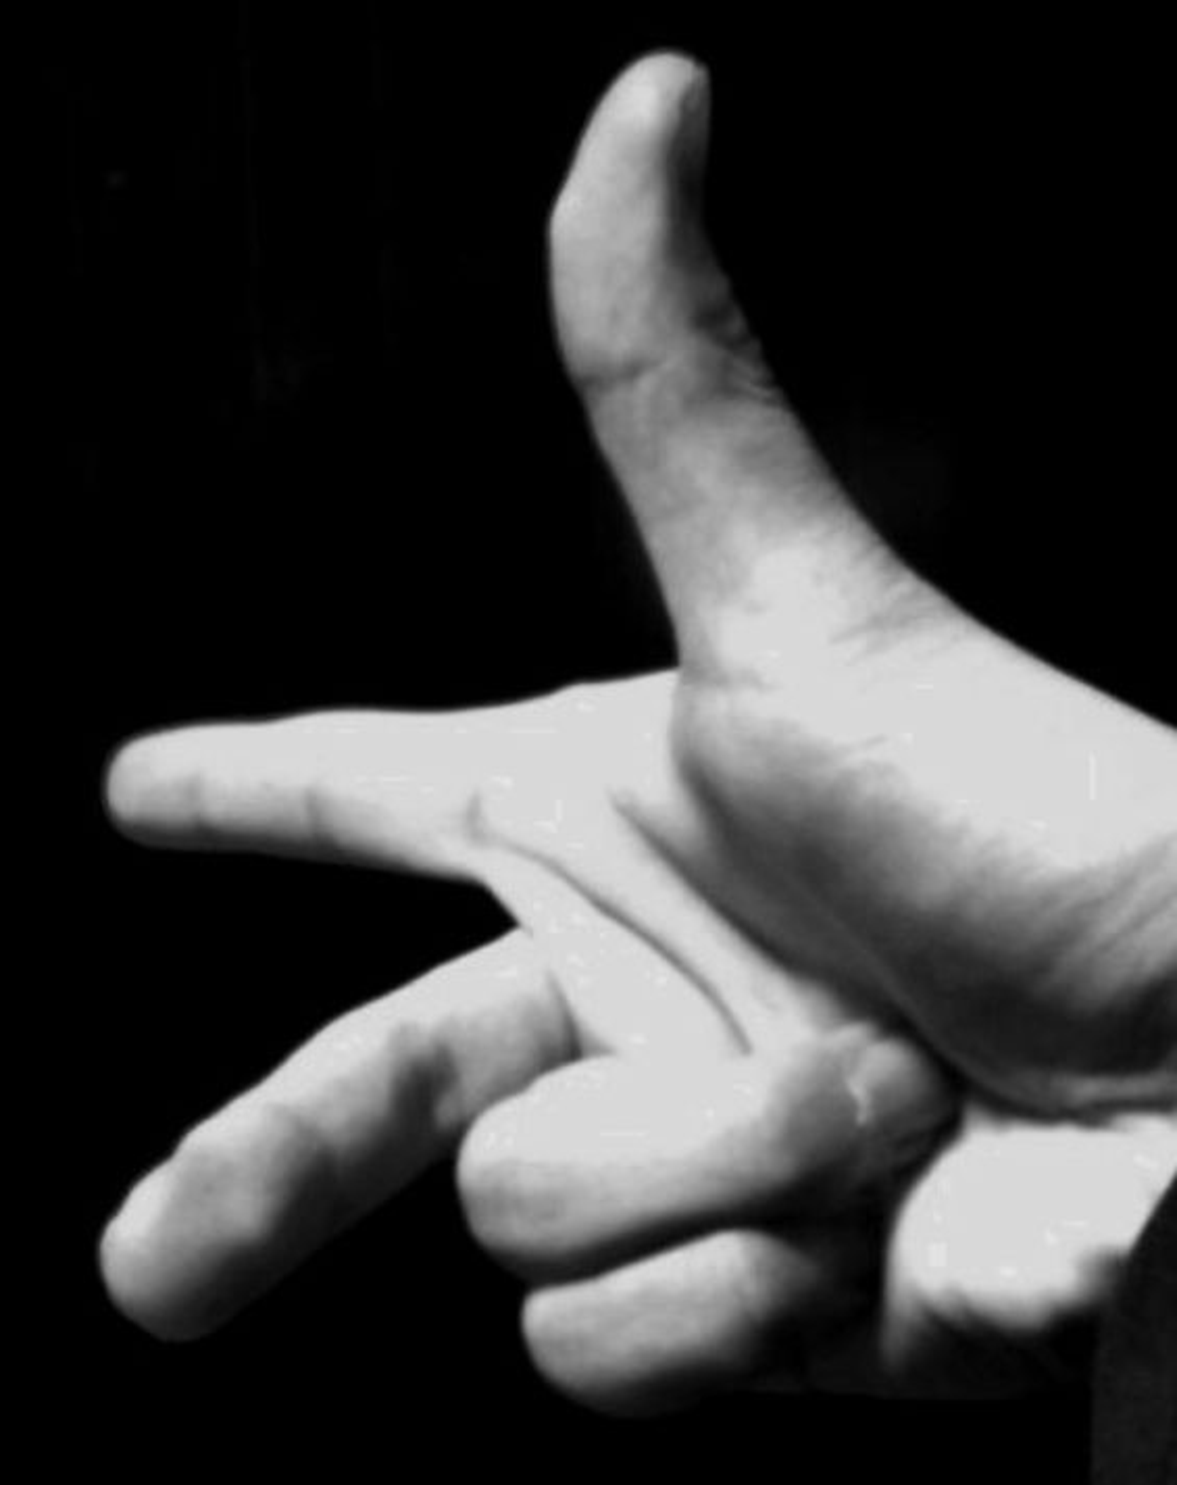
\includegraphics[keepaspectratio, width=3cm,height=3.75cm,clip]{migitekei_TE_mono_x.pdf}

                                    (a) 私の右手
                                    \label{fig:migitekei_TE_mono_x}
                                \end{center}
                            \end{minipage}
                            \begin{minipage}{0.5\hsize}
                                \begin{center}
                                    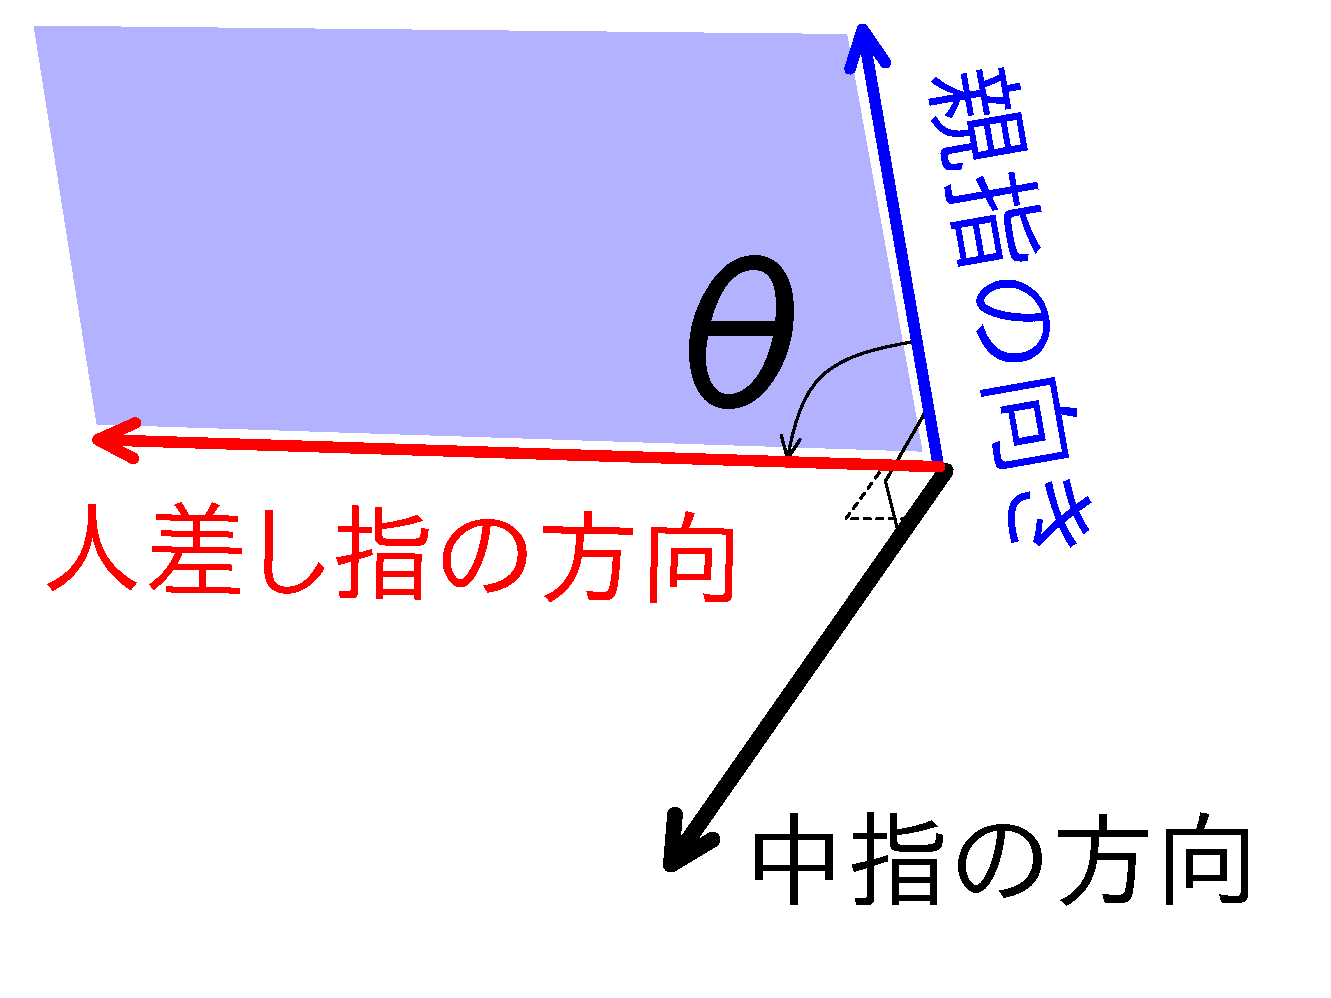
\includegraphics[keepaspectratio, width=3cm,height=3.75cm,clip]{migineji_Myhand.pdf}

                                    (b) 対応図
                                    \label{fig:migineji_Myhand}
                                \end{center}
                            \end{minipage}
                        \end{tabular}
                        \caption{右手系}
                    \end{figure}

                    \begin{figure}[hbt]
                        \begin{center}
                            \includegraphicslarge{VecKagenjoujo.pdf}
                            \caption{ベクトルの和$\cdot$差/$\cdot$積(内積/外積)}
                            \label{fig:VecKagenjoujo}
                        \end{center}
                    \end{figure}
                \end{memo}


%   %==========================================================================
%   %  Section : 特殊なベクトル
%   %==========================================================================
        \section{特殊なベクトル}
%       %----------------------------------------------------------------------
%       %  Input
%       %    File Name : PhysNote_Math_Vector_TaniVector.tex
%       %    説明      : 単位ベクトル,ベクトルの基底などを説明する
%       %----------------------------------------------------------------------
        %   %==========================================================================
%   %  Section : 特殊なベクトル
%   %==========================================================================
        %==================================================================
        %  SubSection
        %==================================================================
            \subsection{単位ベクトル}
                ベクトルは,大きさと向きをもつ.しかし,ベクトルを成分
                表示したときに,その大きさと向きが同時に記述されていて,
                成分表示を見ただけでは,簡単にはその大きさや向きを把握
                することはできない
                    \footnote{
                        計算(暗算)が非常に得意な人や,ベクトルのスペシャリスト
                        でない限り,ベクトルの成分表示を見た瞬間に,その大きさと
                        向きが想像できることはないと思う.少なくとも,私はそのような
                        マネはできない.
                    }.
                そこで,登場するのが,\textbf{単位ベクトル} という概念である.

                自然数でいえば,数字の1がその単位元であり,2以上のすべての自然数は,
                この単位元1の倍数として記述できる.
                    \begin{equation*}
                        2 = 1 \times 2\,,\;3 = 1 \times 3\,,\;\cdots\,.
                    \end{equation*}
                ベクトルの世界では,単位元は1という単なる数値ではなく,
                大きさが1で方向
                    \footnote{
                        「向き」と書いていないことに注意.
                        ここで言っているのは,正の向きと負の向きを同時に
                        考えたいので,「方向」と書いた.
                    }
                をもつ,単位ベクトルという概念が定義される
                    \footnote{
                        定義とは,後の議論の発展のためになされるのであり,
                        導かれるものではない.初学の数学に不慣れである時期には,
                        このことは特に忘れがちである.
                    }.
                    \begin{figure}[hbt]
                        \begin{center}
                            \includegraphicsdefault{TaniVector00.pdf}
                            \caption{単位ベクトル}
                            \label{fig:TaniVector00}
                        \end{center}
                    \end{figure}

                単位ベクトルがあれば,同じ向きを持つベクトルは,その単位ベクトル
                にその大きさをかけることで,ベクトルを表せるのである.
                単位ベクトルと1との違いは,方向をもつか,否かである
                    \footnote{
                        単位ベクトルには方向があり,1には方向がない.
                    }.

                言葉で「単位ベクトル」といったところで,数学的に扱う
                事はできない.なので,単位ベクトルを文字で表そう.

                まだ,単位ベクトルが定義可能か否かは分からないが,
                単位ベクトルなるものがあると仮定して,それを $\bn$ と書くことと
                する.この単位ベクトルを用いると,$\bn$ と同じ方向をもつベクトル
                ならば,$\bn$ の実数倍で表現できる.例えば,ベクトル $\ba$ の向きが
                単位ベクトル $\bn$ と同じ方向であったなら,
                    \begin{equation*}
                        \ba = | \ba | \bn
                    \end{equation*}
                と書ける.これは $\bn$ と同じ向きを持つ任意のベクトルに対して
                成り立つ
                    \footnote{
                        当然,$\bn$ と向きが異るベクトルはこのように記述はできない.
                        その場合には新たに,その方向をもつ別の単位ベクトルを作らないと
                        いけない.つまり,単位ベクトルはその方向によって無数に存在する.
                        これも,自然数の単位元1との違うところだ.
                    }.
                上式を $\bn$ について解くと,
                    \begin{align}
                        \bn = \frac{\ba}{|\ba|}
                    \end{align}
                なる.だから,単位ベクトルとは,ベクトルを自身の大きさで割ったものである
                といえよう.

                念のため,成分表示もしておこう.
                    \begin{align*}
                        \bn &= \frac{\ba}{|\ba|} \\
                            &= \left(
                                    \,\frac{a_{1}}{|\ba|}\,,\,
                                    \,\frac{a_{2}}{|\ba|}\,,\,
                                    \,\frac{a_{3}}{|\ba|}\,\,
                               \right) \\
                            &= \left(
                                    \,\frac{a_{1}}{\sqrt{{a_{1}}^{2}+{a_{2}}^{2}+{a_{3}}^{2}}}\,,\,
                                    \,\frac{a_{2}}{\sqrt{{a_{1}}^{2}+{a_{2}}^{2}+{a_{3}}^{2}}}\,,\,
                                    \,\frac{a_{3}}{\sqrt{{a_{1}}^{2}+{a_{2}}^{2}+{a_{3}}^{2}}}\,\,
                               \right).
                    \end{align*}

                これは大きさが1であり,$\ba$ と同じ方向のベクトルである.なぜなら,ベクトルの
                成分を全てを同じ実数で割ったベクトルと,元のベクトルの方向は同一であることは,
                ベクトルの加減乗除の定義によって簡単に示せる.また,大きさも次の計算から,
                簡単に1であることも確かめられる.
                    \begin{align*}
                        |\bn| &= \left(\frac{a_{1}}{\sqrt{{a_{1}}^2+{a_{2}}^2+{a_{3}}^2}}\right)^{2} +
                                 \left(\frac{a_{2}}{\sqrt{{a_{1}}^2+{a_{2}}^2+{a_{3}}^2}}\right)^{2} \\
                              &\quad + \left(\frac{a_{3}}{\sqrt{{a_{1}}^2+{a_{2}}^2+{a_{3}}^2}}\right)^{2} \\
                              &= \frac{{a_{1}}^{2}+{a_{2}}^{2}+{a_{3}}^{2}}{\left(\sqrt{{a_{1}}^2+{a_{2}}^2+{a_{3}}^2}\right)^{2}} \\
                              &= \frac{{a_{1}}^{2}+{a_{2}}^{2}+{a_{3}}^{2}}{{a_{1}}^2+{a_{2}}^2+{a_{3}}^{2}} \\
                              &= 1 \\
                        \therefore\quad
                        |\bn| &= 1.
                    \end{align*}

                \begin{memo}{具体例}
                    ベクトル $\ba=\left[\,1,\,2,\,4\,\right]$ を,大きさと
                    単位ベクトルに分解してみよう.

                    まず大きさは,定義に従って
                        \begin{equation*}
                            |\ba| = \sqrt{1^{2}+2^{2}+4^{2}} = \sqrt{1+4+16} = \sqrt{21}
                        \end{equation*}
                    である.よって,求めたい単位ベクトルを $\bn$ と書くことにすれば,
                        \begin{equation*}
                            \bn = \frac{\ba}{|\ba|} = \frac{1}{\sqrt{21}}\left[\,1,\,2,\,4\,\right]
                                = \left[
                                    \,\frac{1}{\sqrt{21}},\,\frac{2}{\sqrt{21}},\frac{4}{\sqrt{21}}\,
                                  \right].
                        \end{equation*}

                    以上から,ベクトル $\ba$ は大きさと単位ベクトルに分解すると,
                        \begin{equation*}
                            \ba = |\ba|\bn = \sqrt{21}
                                  \left[
                                    \,\frac{1}{\sqrt{21}},\,\frac{2}{\sqrt{21}},\frac{4}{\sqrt{21}}\,
                                  \right]
                        \end{equation*}
                    と表現される.
                \end{memo}

        %==================================================================
        %  SubSection
        %==================================================================
            \subsection{基底ベクトル}
                先に単位ベクトルという概念を説明した.そして,ここでは
                単位ベクトルを使って,さらに新し考え方を導入する.

                いきなりだけど,具体例から考える.
                ひとつの任意のベクトル $\ba$ を
                もってきて,$\ba$ が次のようなベクトルだったとしよう
                    \footnote{
                        まずは,馴染み深い3次元ベクトルで考える.
                    }.
                    \begin{equation*}
                        \ba
                        =
                        \left[
                            \begin{array}{c}
                                1 \\
                                3 \\
                                5 \\
                            \end{array}
                        \right].
                    \end{equation*}
                この式は次のように見ることもできる.
                    \begin{equation*}
                        \ba
                        =
                        1\left[
                            \begin{array}{c}
                                1 \\
                                0 \\
                                0 \\
                            \end{array}
                        \right]
                        +
                        3\left[
                            \begin{array}{c}
                                0 \\
                                1 \\
                                0 \\
                            \end{array}
                        \right]
                        +
                        5\left[
                            \begin{array}{c}
                                0 \\
                                0 \\
                                1 \\
                            \end{array}
                        \right].
                    \end{equation*}
                3つの方向に対し,ひつの方向に1の大きさをもち,かつ,
                他の方向には0であるような単位ベクトルを作り,
                それに係数をかけて,足し合わせるのである.

                任意のベクトルに対して,この表し方が可能であることは,
                明白である.任意の $n$ 次元ベクトル $\bx$ が
                    \begin{equation*}
                        \bx
                        =
                        \left[
                            \begin{array}{c}
                                x_{1} \\
                                x_{2} \\
                                \vdots \\
                                x_{n} \\
                            \end{array}
                        \right].
                    \end{equation*}
                と成分表示されるとしよう.このとき,$\bx$ は
                次のようにも表現することが可能である.
                    \begin{equation*}
                        \bx
                        =
                        x_{1}\left[
                            \begin{array}{c}
                                1 \\
                                0 \\
                                0 \\
                                0 \\
                                \vdots \\
                                \vdots \\
                                0 \\
                            \end{array}
                        \right]
                        +
                        x_{2}\left[
                            \begin{array}{c}
                                0 \\
                                1 \\
                                0 \\
                                0 \\
                                \vdots \\
                                \vdots \\
                                0 \\
                            \end{array}
                        \right]
                        +
                        \cdots
                        +
                        x_{i}\left[
                            \begin{array}{c}
                                0 \\
                                \vdots \\
                                0 \\
                                1 \\
                                0 \\
                                \vdots \\
                                0 \\
                            \end{array}
                        \right]
                        +
                        \cdots
                        +
                        x_{n}\left[
                            \begin{array}{c}
                                0 \\
                                0 \\
                                0 \\
                                \vdots \\
                                \vdots \\
                                0 \\
                                1 \\
                            \end{array}
                        \right]
                        .
                    \end{equation*}

                    このような書き方だと,記述が少々面倒なので,
                    次のような記号を導入し,表現を簡略化させよう.
                    \begin{align}
                        \be_{1}
                        =
                        \left[
                            \begin{array}{c}
                                1 \\
                                0 \\
                                0 \\
                                0 \\
                                \vdots \\
                                \vdots \\
                                0 \\
                            \end{array}
                        \right]
                        \; , \;
                        \be_{2}
                        =
                        \left[
                            \begin{array}{c}
                                0 \\
                                1 \\
                                0 \\
                                0 \\
                                \vdots \\
                                \vdots \\
                                0 \\
                            \end{array}
                        \right]
                        \; , \cdots , \;
                        \be_{i}
                        =
                        \left[
                            \begin{array}{c}
                                0 \\
                                \vdots \\
                                0 \\
                                1 \\
                                0 \\
                                \vdots \\
                                0 \\
                            \end{array}
                        \right]
                        \; , \cdots , \;
                        \be_{n}
                        =
                        \left[
                            \begin{array}{c}
                                0 \\
                                0 \\
                                0 \\
                                \vdots \\
                                \vdots \\
                                0 \\
                                1 \\
                            \end{array}
                        \right].
                    \end{align}

                    このように,一成分が1であり,他の成分がすべて0であるようなベクトルを,
                    \textbf{基底ベクトル} という.もちろん,基底ベクトルとは,
                    任意のベクトルを表現する場合に用いるベクトルである.しかし,たまたま任意の
                    ベクトルが基底ベクトルの成分と一致してしまうこともある.この場合のベクトルは
                    基底ベクトルとは認識されない.

                    基底ベクトルという概念を使うと,$\bx$ は以下のように書き直せる.
                        \begin{align}
                            \bx = x_{1}\be_{1} + x_{2}\be_{2} + \cdots + x_{i}\be_{i} + \cdots + x_{n}\be_{n}.
                        \end{align}

                    和の記号 $\sum_{i=1}^{n}$ を使うともっと簡単になる.
                        \begin{align}
                            \bx = \sum_{i=1}^{n} x_{i}\be_{i}.
                        \end{align}

                    \begin{memo}{注意}
                        基底ベクトルを先に「一成分が1であり,他の成分がすべて0であるようなベクトル」と
                        定義してしまった.しかし,注意してほしい.より細かく言うと,“直線直交座標系”における
                        基底ベクトルと表現すべきであった.

                        基底ベクトルは,座標系によってことなる.座標系には,直線直交座標意外にも,
                        極座標系や円筒座標系
                            \footnote{
                                後で説明する.中学から使ってきた,$x$--$y$ 座標のことを,直線直交座標というが,
                                これ以外にも,上に書いたように,極座標系や円筒座標系など,様々な座標系を設定
                                できる.ここでは,座標系は直線直交座標系だけではないということを
                                分かってもらえれば,それでいい.
                            }
                        があり,各座標系の基底ベクトルは全く異なるベクトルである
                            \footnote{
                                ただし,ある基底ベクトルが存在するとき,この基底ベクトルを別の基底ベクトル
                                に変換する方法は存在する.
                            }.
                    \end{memo}
